\subsection{Getting verbose!}

Although we use colours in SDMs to indicate when an element is to be matched (black), created (green), or destroyed (red), sometimes, especially for a black and
white printout, it makes sense to indicate this via explicit stereotypes.

\begin{enumerate}
\item[$\blacktriangleright$] Right�click on a diagram and select ''Extensions/extras/Set Moflon::Verbose to true'' to enable \texttt{<<create>>} and
\texttt{<<destroy>>} stereotypes (Fig.~\ref{fig_usingVerbose01}).

\item[$\blacktriangleright$] You can hide the stereotypes again by selecting ``Extensions/extras/Set Moflon:: Verbose to false''
(Fig.~\ref{fig_usingVerbose01}).

\begin{figure}[htbp]
\begin{center}
  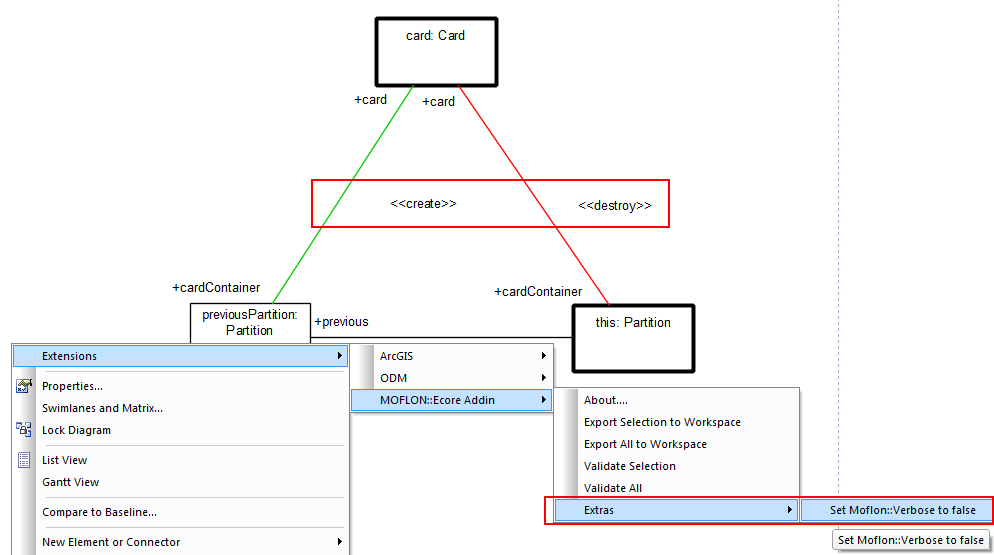
\includegraphics[width=0.9\textwidth]{usingVerbose1}
  \caption{Verbal change of links}  
  \label{fig_usingVerbose01}
\end{center}
\end{figure}
\end{enumerate}